\section{Introduction}
% \begin{framed}

% * Introduce EDA based solution from advantages point of view, highlight no overheads, design freedom ( select only gates that have no impact on area,power and delay). re-pitch paragraph 3 .

% * Show none of current EDA flows consider security.

% * Change references, use standard ones and include PC based references.

% * Include figure for indicating hotspots.

% * Move marked paragraph to overview section

% \end{framed}
% \begin{framed}
% 1. Introduction: Add a contributions section.\\
% 2. Background and Literature Survey: Let the literature review be cursory. Elaborate treatment must be written in separate section. Introduce Security -- TVLA, CPA, DPA, Differential and Correlational power analysis; Leakage power optimization -- Vt sizing, gate sizing, Vdd scaling, \\
% 3. Add a Motivation Section -- Highlight the results of the following experiments: (1) Effect of each design optimization on the security of the gate; (2) It is possible to measure this impact at the design stage itself.
% 4. High Level Overview. -- Introduce the high-level components of your solution using a flow chart. \\
% 5. Proposed Solution -- Elaborate on the components mentioned in the High-Level overview.\\
% 6. Theoretical analysis -- can you come up with optimal size of grids. See if effect of design choices on security can be modeled theoretically.\\
% 7. Implementation. -- making the scripts open source. \\
% 8. Experiments -- TBD
% \end{framed}

% We live in a connected world today. This has largely been made possible due to the advent of an era of connected systems that seamlessly interact with each other thereby reducing the load on us. This network, largely referred to as Internet of Things, makes use of small, low cost devices or embedded systems. In the last five years over 5 billion devices have been deployed. 

% The ubiquity of IoT means that, of late these devices are entrusted with the responsibility of i) storing sensitive data such as personal information, financial information or medical history in order to improve the quality of our life or ii) using sensitive data in order perform a specific task such as heart rate monitors, password devices etc. At this stage it is important to ask the question "Can these devices be trusted?". 


% Figure~\ref{fig:stack} shows the various levels of the system stack. These parts seamlessly interact in order for an application to run, however a violation or misinterpretation of the specification at any level might provide a potential entry point through which the attacker can access sensitive data. It has been shown that time and again these devices have been exploited either through vulnerabilities at the software level or at the hardware level. This has led researchers to focus on developing mechanisms that try and prevent such vulnerabilities from being exploited or identifying novel vulnerabilities. 




% It has been shown time and again that these devices can be exploited. The reason for these attacks can be at any level of  by using vulnerabilities existing at various levels of the system stack, ranging from end-user applications to the underlying hardware on which these applications run. Side-channel attack is one such attack that exploits the vulnerability in the hardware of these embedded devices. %{\color{red}Not all hardware attacks are side-channel based, no? Response: I meant all side-channel attacks are hardware attacks..the reverse may or not be true.}

Electronic devices today need to simultaneously meet  stringent requirements of area, power, performance, and security. While all commercially available Electronic Design Automation (EDA) tools provide several optimizations to meet the former three design requirements, most do not have any provisions to address the security requirements of a device. One important security requirement, especially for embedded devices, is to limit the side-channel leakage through the device's power consumption. These leakages, if present, provide clues about the internal computation being performed in the device and  have been used to break crypto-algorithms~\cite{kocher:99} and to reverse engineer software~\cite{park:2018}.

 Most designs address side-channel leakage requirements of a device at the algorithm level by randomizing computations, which  in turn randomizes its side-channel leakage~\cite{akkar:2001}. Other schemes work at the system level by injecting noise in the power supply, which reduces the signal-to-noise ratio in the side-channel leakage~\cite{Wang:2013,tokunaga:2009,singh:2015,mathew:2018}. Both these schemes require specialized circuitry which can drastically affect the area, power, and performance of the design. For example, the  popular algorithmic masking scheme ~\cite{canright}, results in performance degradation of over $3\times$. 

%power attacks attempt to either eliminate leakage or randomize it. Most common randomization procedures rely on algorithmic techniques to mask the leakage~\cite{akkar:2001}, while  elimination countermeasures employ specialized gates or transistors to nullify the leakage~\cite{Tiri:2004}. Both these types of countermeasures incur significant overheads in performance, area and power. For example, a typical elimination countermeasure increases chip delay  by $42\%$ and the area overheads by $3.5\times$~\cite{Tiri:2004}. These overheads are not always acceptable for embedded systems, where area and power are highly constrained.

\begin{figure}[!t]
 \centering
  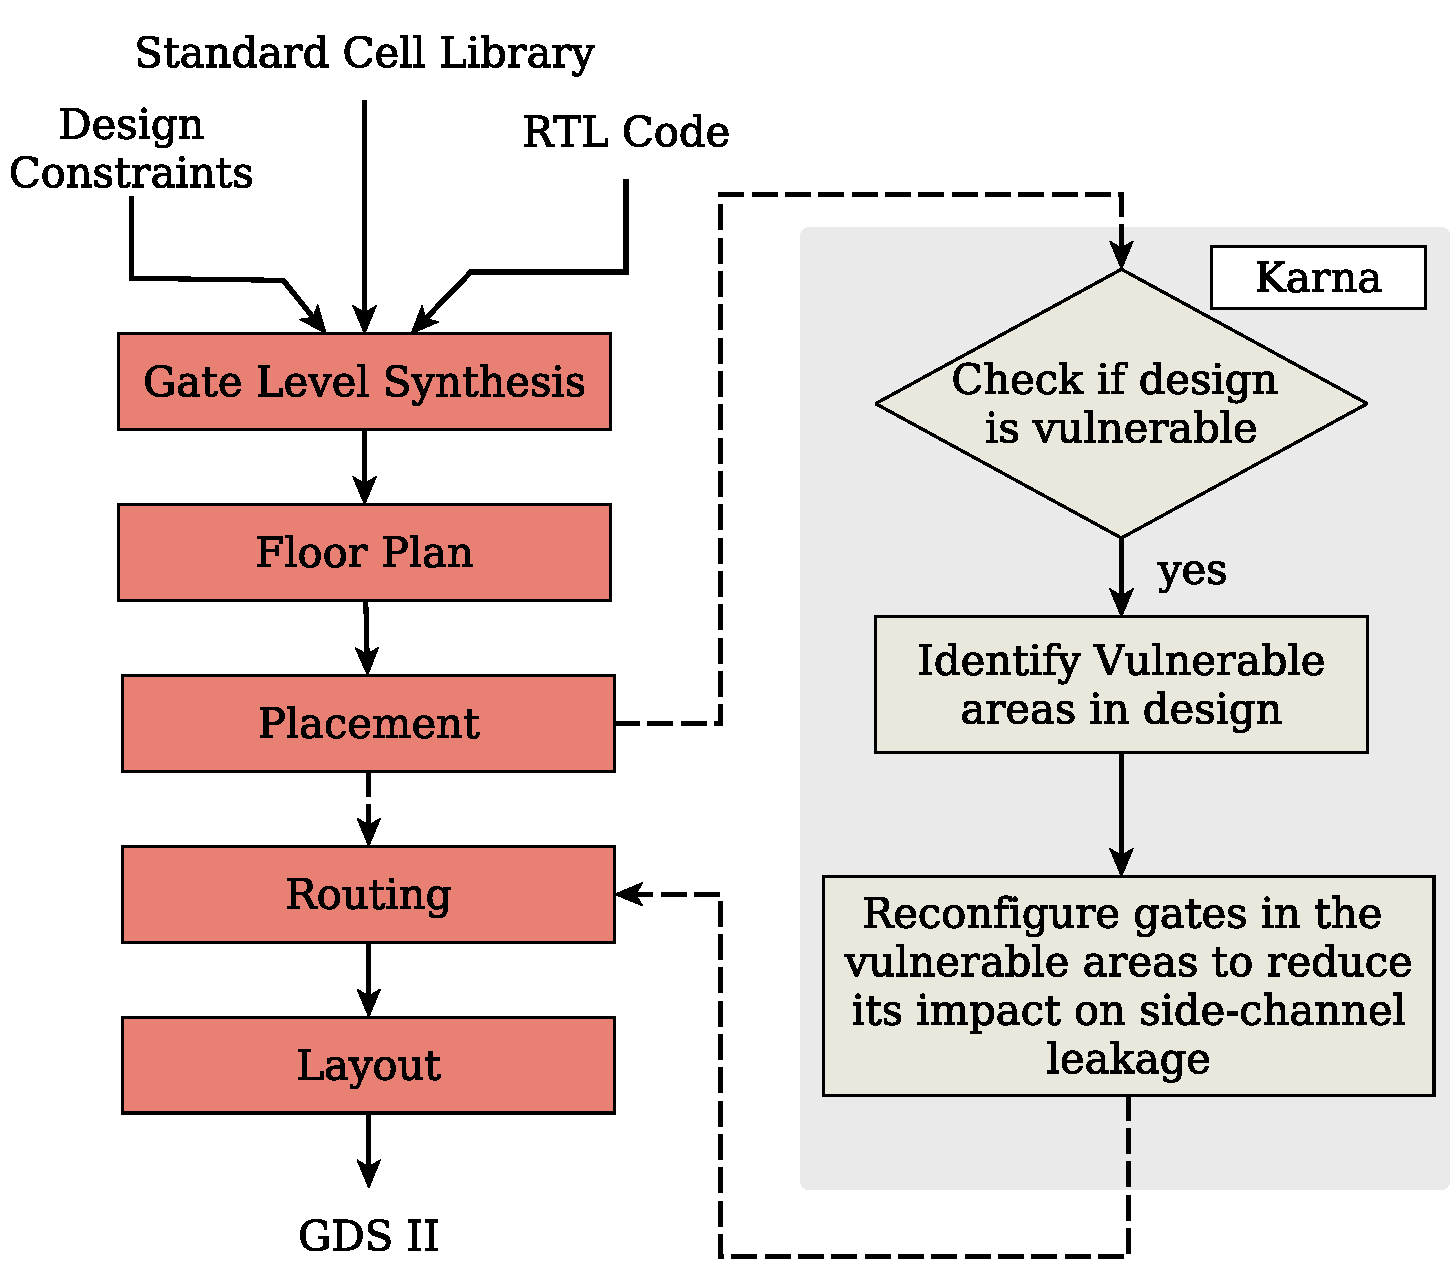
\includegraphics[scale=0.33]{Chapter4/karna.pdf}
  \caption{Figure showing the integration of {\sf Karna} into a standard EDA flow. The {\sf Karna} module inserted in the EDA flow is used to achieve side-channel security while still honoring the design's requirements in area, power, and performance.}
  \label{fig:vlsiflow}
  \vspace{-15pt}
\end{figure}

In this paper, we propose to address the side-channel security requirements of a design through the EDA flow, while still meeting other design requirements of area, power, and performance. We introduce a module called \textsf{Karna} in the EDA flow, that takes the user-specified security level as input and optimizes the parameters of the gates in the placed netlist until the desired side-channel security is achieved (Figure~\ref{fig:vlsiflow}). No specialized circuits to counter side-channel attacks are introduced during the process. The design of \textsf{Karna} is based on two critical observations. First, there are some regions in the design which contribute much more significantly to the side-channel leakage than other regions. It is sufficient to focus on these vulnerable regions in order to reduce side-channel leakage. Second, the gate-level parameters such as supply voltage, threshold voltage, and the gate size can influence the amount of side-channel leakage. 
Carefully selecting these gate-level parameters can therefore reduce side-channel leakage of the gate. 
At a high level, {\sf Karna} first identifies vulnerable regions in the design and then reconfigures the gate parameters present in these regions such that the overall side-channel leakage of the design is reduced. 
%{\sf Karna} is designed to not just achieve the security objectives of the design but also  achieve the other design objective such as area, power and performance.  


 In 2005, Tiri et al.~\cite{Verbauwhede:2005} also proposed changes to the EDA flow to prevent side-channel leakage. 
However, their scheme requires specialized gate libraries, that are not always supported by the foundry, and can considerably affect other device parameters. For example, the area of the side-channel protected AES design in~\cite{Verbauwhede:2005} increases by $3.4\times$, while the energy requirement increase by $5.9\times$. {\sf Karna}, on the other hand uses gates available in the standard cell library, and configures parameters like supply voltage, threshold voltage, and size of the vulnerable gates in order to reduce the side-channel leakage in the design phase thereby minimizing the overheads. In our work we demonstrate, using three cipher, that the area and performance and power consumption of the  designs passed through {\sf Karna} is not affected, while the side-channel leakage reduces.
The contributions of this paper are as follows.
\begin{itemize}[leftmargin=1pc]
\item We incorporate {\sf Karna} into the Synopsys design flow {M-2016 12-SP5-4} in order to pinpoint the regions in a placed netlist that contribute significantly to the side-channel leakage. 
\item We incorporate a gate-level power-optimization algorithm, which considers the side-channel security objectives of the design along with the standard design constraints such as area, power and delay.
\item {\sf Karna} provides a tunable parameter by which side-channel security can be traded off with design effort.
\item We test the efficacy of {\sf Karna} on three block cipher implementations: AES, PRESENT, and Simon. Each implementation is synthesized for a 28nm technology node. We demonstrate each design's side-channel resistance using the Test Vector Leakage Assessment (TVLA) metric~\cite{becker:2013} and show that the TVLA scores are less than 4.5 even after 100,000 measurements, while the original design requirements of power, area, and performance are unaffected.
 \end{itemize}

\noindent The outline of the paper is as follows: we introduce the necessary terminology in Section~\ref{sec:background}, motivate the need for {\sf Karna} in Section~\ref{sec:motivation} and describe it in Section~\ref{sec:proposed}. The experimental setup and results are presented in Section~\ref{sec:experiment}. The related work is discussed in Section~\ref{sec:related} and Section~\ref{sec:conclusion} concludes the paper by describing the future directions.









% \todo[inline]{can be moved to discussion section}
% Introducing security optimizations at the earlier stage of the design could cause the subsequent stages in the EDA flow to optimize or remove the changes and thereby render them useless~\cite{danger:2017}. We take into account these two constraints and integrate {\sf Karna} at the post-placement stage in the EDA flow where the delay, power and area of the design can be accurately estimated and also ensuring that the security changes are carried over into the manufactured device.


% Compared to contemporary  countermeasures~\cite{yang:2005,Singh:2017,Wang:2013,Yu:2015}, which ensure security of a manufactured device, our EDA based approach would enable fine-grained control by inserting countermeasures at the design stage itself. Further, unlike other countermeasures, which either require additional operations or new circuitry to be added, our EDA based approach would not have any such overheads. Our solution leverages the fact that EDA tools work at the gate level, which provides several tunable options like the gate's threshold voltage, size, supply voltage and load capacitance thereby enabling the design to meet a wider range of security objectives. 

%The motivation for using EDA tools for countering power analysis attacks is due to the observation that not all areas of the design contribute to the side-channel leakage. Thus, there is scope for EDA tools to optimize vulnerable regions for security. %should talk about observation
%As an example, consider Figure~\ref{fig:aes} which shows that not all areas of an AES design contribute equally to the side-channel leakage. 



%The methodology of using EDA tools to achieve side-channel security has been addressed in~\cite{Tiri:2005} where the authors introduce specialized libraries to mitigate side-channels. While this scheme efficiently eliminates side-channel leakage from the device it incurs a huge area overhead of 4$\times$~\cite{}. Our proposed scheme, on the other hand, uses the standard cell library and therefore does not incur any overheads. We achieve security by efficiently configuring the available gates.

% . The amount of effort required to characterize the library for security is very high. The points are
% \begin{itemize}
% \item Each gate is characterized for multiple corners and multiple modes so a secure library should be available for each corner and mode
% \item Number of gates increases with each node ( 330 in 32nm to 660 in 28nm).
% \item Area and delay overheads
% \item Library characterization places reliance on the foundry, no way to verify if the gate actually secures the design.
% \end{itemize}
% significant advantages over existing countermeasure techniques. 

%In this paper, we propose {\sf Karna}, a security aware module that reduces the side-channel leakage of a design. A user enables the module and specifies the desired level of security using a \texttt{security\_level} option. A high security level will cause the module to aggressively optimize the design for security. Thus a higher security level would imply a higher resistance to power analysis attacks.

%\textbf{Marked} typical EDA flow consists of several stages as shown in Figure~\ref{fig:vlsiflow}. Each stage in the flow has a specific objective to optimize one or more of the delay, power or area. The modules at each stage rely on timing and power models of the gates to achieve their objective. An EDA flow, which is security aware,  can address this objective in multiple stages. This choice can affect the other design constraints such as area, performance, and power. For example, countermeasures such as masking is incorporated in the stage 1, the high-level description stage, while gate level schemes on the other hand is incorporated in stage 2, the gate level synthesis level. Incorporating security at these stages might cause the design to incur delay and area overheads leading to the design not meeting the required area and timing constraints in the subsequent stages. Further, incorporating security in the early stages may get undone by subsequent stages. In this work, we therefore choose to introduce the {\sf Karna} module after the design is placed. At this stage, a realistic estimation of the interconnect delay and power density is known. Thus, in this stage, we can accurately gauge the impact of the proposed security based modifications on the area, delay, and performance of the device. 


%

%This security aware EDA flow is validated using an AES-128 netlist synthesized at 28nm technology. We verify the impact of our proposed flow on the area, power and delay constraints using the Synopsys Design Compiler.


